% Figura Anexo I: derivación de la curva LM desde el mercado de dinero y sus tres tramos
\documentclass[tikz,border=3pt]{standalone}
\usepackage[T1]{fontenc}
\usepackage[utf8]{inputenc}
\usetikzlibrary{arrows.meta,calc,decorations.pathreplacing}
\begin{document}
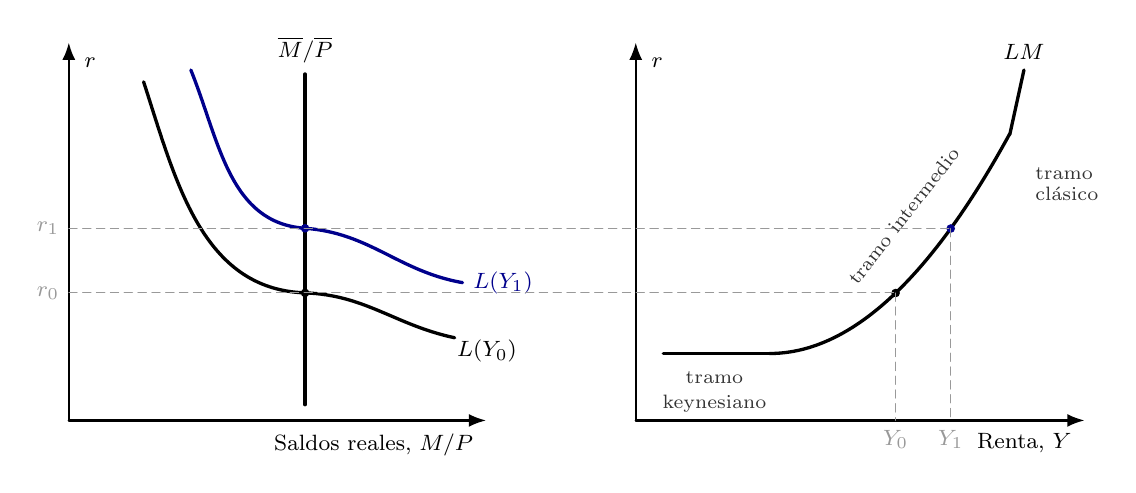
\begin{tikzpicture}[>={Latex[length=2.2mm]}, line cap=round, font=\footnotesize,
  eje/.style={->, thick},
  curva/.style={very thick},
  nueva/.style={very thick, blue!55!black},
  guia/.style={densely dashed, gray!80},
  pto/.style={circle, fill=black, inner sep=1.1pt}]
  % ---------- Panel izquierdo: mercado de dinero ----------
  \draw[eje] (0,0) -- (5.3,0) node[below left=1pt]{Saldos reales, $M/P$};
  \draw[eje] (0,0) -- (0,4.8) node[below right=2pt]{$r$};
  \draw[curva] (3,0.2) -- (3,4.4) node[above]{$\overline{M}/\overline{P}$};
  \draw[curva] (0.95,4.3) to[out=-72,in=178] (3,1.62) to[out=-2,in=168] (4.9,1.05) node[below right=-3pt]{$L(Y_0)$};
  \draw[nueva] (1.55,4.45) to[out=-68,in=176] (3,2.44) to[out=-4,in=170] (5.0,1.75) node[right]{$L(Y_1)$};
  \node[pto] at (3,1.62) {};
  \node[pto, fill=blue!55!black] at (3,2.44) {};
  % ---------- Panel derecho: curva LM ----------
  \begin{scope}[xshift=7.2cm]
    \draw[eje] (0,0) -- (5.7,0) node[below left=1pt]{Renta, $Y$};
    \draw[eje] (0,0) -- (0,4.8) node[below right=2pt]{$r$};
    % LM: tramo plano + tramo creciente (r = 0,85 + 0,3 (Y-1,7)^2) + tramo vertical
    \draw[curva] (0.35,0.85) -- (1.7,0.85);
    \draw[curva] plot[domain=1.7:4.75, samples=50] (\x,{0.85+0.3*(\x-1.7)^2});
    \draw[curva] (4.75,3.63) -- (4.93,4.45) node[above]{$LM$};
    \node[pto] at (3.3,1.618) {};
    \node[pto, fill=blue!55!black] at (4.0,2.437) {};
    \draw[guia] (3.3,1.618) -- (3.3,0) node[below]{$Y_0$};
    \draw[guia] (4.0,2.437) -- (4.0,0) node[below]{$Y_1$};
    % Tramos
    \node[below, gray!40!black] at (1.0,0.75) {\scriptsize tramo};
    \node[below, gray!40!black] at (1.0,0.45) {\scriptsize keynesiano};
    \node[gray!40!black, rotate=52] at (3.4,2.6) {\scriptsize tramo intermedio};
    \node[gray!40!black, right, align=left] at (4.95,3.0) {\scriptsize tramo\\[-2pt]\scriptsize clásico};
  \end{scope}
  % Guías horizontales comunes (mismo tipo de interés en ambos paneles)
  \draw[guia] (0,1.62) node[left]{$r_0$} -- (10.5,1.62);
  \draw[guia] (0,2.44) node[left]{$r_1$} -- (11.2,2.44);
\end{tikzpicture}
\end{document}
